\title{Aula 4 - Conceitos Básicos de Segurança da Informação}

\author{Prof. Gabriel Rodrigues Caldas de Aquino}

\institute
{
    Instituto de Computação \\
    Universidade Federal do Rio de Janeiro\\
    gabrielaquino@ic.ufrj.br % Your institution for the title page
}
\date{Compilado em: \\ \today} % Date, can be changed to a custom date

%----------------------------------------------------------------------------------------
%    PRESENTATION SLIDES
%----------------------------------------------------------------------------------------


\begin{frame}
    % Print the title page as the first slide
    \titlepage
\end{frame}








\begin{frame}{Três pilares da Segurança da informação}

    Os três pilares da segurança da informação são:

    \begin{columns}[T]
        \begin{column}{0.32\textwidth}
            \begin{alertblock}{Confidencialidade}
                \footnotesize
                \textbf{Definição:} Proteção contra acesso não autorizado\\
                \textbf{Ameaça:} Vazamento de dados\\
                \textbf{Exemplo:} Sigilo de processos judiciais
            \end{alertblock}
        \end{column}

        \begin{column}{0.32\textwidth}
            \begin{alertblock}{Integridade}
                \footnotesize
                \textbf{Definição:} Prevenção de alterações indevidas\\
                \textbf{Ameaça:} Fraude em registros\\
                \textbf{Exemplo:} Sistemas para eleições
            \end{alertblock}
        \end{column}

        \begin{column}{0.32\textwidth}
            \begin{alertblock}{Disponibilidade}
                \footnotesize
                \textbf{Definição:} Acesso contínuo aos sistemas\\
                \textbf{Ameaça:} Ataques DDoS\\
                \textbf{Exemplo:} Plataforma durante a ataques ou crises
            \end{alertblock}
        \end{column}
    \end{columns}



    Exemplo dos três pilares em um sistema:
    \begin{itemize}
        \footnotesize
        \item Sigilo das transações (Confidencialidade)
        \item Manutenção dos saldos (Integridade)
        \item Operação 24/7 (Disponibilidade)
    \end{itemize}

\end{frame}


\begin{frame}{Extensão dos três pilares: Autenticidade e Não-Repúdio}

    \begin{itemize}
        \item \textbf{Autenticidade e não-repúdio}: Garantia da origem legítima das informações \textbf{e} impossibilidade de negar participação em uma transação.
              \begin{itemize}
                  \item \textbf{Autenticidade}: Propriedade que garante que a origem de uma informação é legítima e verificável.
                  \item  \textbf{Não-repúdio}: Capacidade de provar que uma ação ocorreu e que sua origem não pode ser negada pelas partes envolvidas.\\
              \end{itemize}


    \end{itemize}





\end{frame}

\begin{frame}{Como ter autenticidade mas não ter não-repúdio? - Exemplo 1}
    \textbf{Cenário:} Um usuário preenche um formulário em papel, marcando opções com um “X” e assinando no final.

    \medskip
    \textbf{Autenticidade:}
    A assinatura garante que o formulário foi realmente assinado pelo usuário — \textbf{autenticidade}.

    \medskip
    \textbf{Não-Repúdio:}
    Posteriormente, o usuário alega: ``Eu não marquei estas opções''.
    Como não há registro eletrônico ou prova criptográfica do preenchimento das opções, não é possível contestar a alegação — \textbf{não-repúdio}.

    \medskip
    \textbf{Como garantir não repúdio:}
    \begin{itemize}
        \item Uso de formulários digitais com marcação eletrônica vinculada à assinatura digital.
        \item Registro seguro de cada ação com timestamp, de forma auditável.
    \end{itemize}
\end{frame}


\begin{frame}{Como ter autenticidade sem ter não-repúdio? - Exemplo 2}
    \textbf{Cenário:} Um funcionário envia um pedido de reembolso via e-mail corporativo.

    \medskip
    \textbf{Autenticidade:}
    O e-mail vem de sua conta corporativa e o sistema confirma que ele é o remetente — \textbf{autenticidade}.

    \medskip
    \textbf{Não-repúdio:}
    O funcionário depois alega: ``Eu não enviei este pedido, alguém acessou minha conta''.
    Sem uma assinatura digital ou registro auditável adicional, a empresa não consegue provar de forma incontestável que ele realmente enviou o e-mail — \textbf{não-repúdio}.

    \medskip
    \textbf{Como garantir não-repúdio:}
    \begin{itemize}
        \item Assinatura digital do e-mail ou do pedido.
        \item Logs seguros e auditáveis da ação com timestamp.
    \end{itemize}
\end{frame}


\begin{frame}{Autenticidade e não-repúdio}
    \textbf{Autenticidade} \\
    Propriedade de ser genuíno, verificável e confiável. Envolve ter confiança na validade de uma transmissão, mensagem ou origem da mensagem.
    Verifica se os usuários são quem dizem ser e se cada entrada recebida veio de uma fonte confiável.

    \medskip
    Exemplo:
    \begin{itemize}
        \item Documento manuscrito: comparação das características de escrita com amostras verificadas.
        \item Informação eletrônica: uso de assinatura digital com criptografia de chave pública para verificar autoria e, possivelmente, a integridade.
    \end{itemize}

    \medskip
    \textbf{Não-repúdio} \\
    Capacidade de provar que um evento ou ação ocorreu e qual foi sua origem, evitando que as partes envolvidas neguem posteriormente.
    \begin{itemize}
        \item Prova de entrega para o remetente.
        \item Prova de identidade do remetente para o destinatário.
    \end{itemize}
\end{frame}

\begin{frame}{Exemplo: Assinatura Digital via ITI (ICP-Brasil)}
    \textbf{Cenário:} Assina digital de documento utilizando o assinador do ITI \href{https://www.gov.br/iti/pt-br}{\textcolor{blue}{(Link)}}
    Usando a Infraestrutura de Chaves Públicas (ICP) (\href{https://www.gov.br/iti/pt-br/assuntos/icp-brasil}{\textcolor{blue}{ICP-Brasil}}).


    \begin{itemize}
        \item Certificado digital vinculado à identidade do usuário.
        \item Chave privada usada para assinar digitalmente o documento.
        \item Registro auditável da assinatura.
        \item Verificação automática de alterações posteriores ao documento assinado.
    \end{itemize}

    \medskip
    \textbf{Autenticidade:}
    O sistema verifica que a assinatura foi feita pelo titular do certificado digital ou pela conta \textit{gov.br}
    — \textbf{autenticidade}.

    \medskip
    \textbf{Não-Repúdio:}
    Assinatura feita com a chave privada do usuário e registrada no site do ITI (\href{https://assinador.iti.br}{Assinador ITI}), o usuário \textbf{não pode negar posteriormente} que assinou o documento — \textbf{não repúdio}.

    \medskip
    \textbf{Integridade:}
    Se alguém tentar alterar o documento após a assinatura, o sistema detecta que ele foi modificado, garantindo que o conteúdo original permanece inalterado.



\end{frame}



\begin{frame}{Autenticidade e Não-Repúdio}
    \begin{block}{Autenticidade}
        \begin{itemize}
            \item Garante que a mensagem ou ação veio realmente de quem afirma tê-la realizado.
            \item Exemplos:
                  \begin{itemize}
                      \item Login com senha ou biometria.
                      \item Certificado digital em sites HTTPS.
                      \item Assinatura digital para verificação do remetente.
                  \end{itemize}
        \end{itemize}
    \end{block}

    \begin{block}{Não-Repúdio}
        \begin{itemize}
            \item Impede que o autor de uma ação negue sua responsabilidade posteriormente.
            \item Exemplos:
                  \begin{itemize}
                      \item Assinaturas digitais com certificado ICP-Brasil.
                      \item Registros assinados de transações financeiras.
                      \item Logs de auditoria assinados digitalmente.
                  \end{itemize}
        \end{itemize}
    \end{block}
\end{frame}


\begin{frame}{Extensão dos três pilares: Responsabilização (Accountability)}

    \begin{itemize}
        \item \textbf{Definição de Accountability:} Segurança que exige que ações de uma entidade sejam rastreadas exclusivamente para ela.
        \item \textbf{Objetivos de Accountability:}
              \begin{itemize}
                  \item Suportar o \textbf{não repúdio}.
                  \item Prevenir ou desencorajar \textbf{comportamentos indesejados}
                  \item Promover  \textbf{isolamento de falhas}.
                  \item \textbf{Detectar e prevenir de intrusões}.
                  \item Facilitar a \textbf{recuperação após ação} e apoio para ações legais.
              \end{itemize}
        \item \textbf{Importância:}
              \begin{itemize}
                  \item Permite rastrear brechas de segurança até a parte responsável.
                  \item Registros de atividades são fundamentais em uma para análise forense.
                  \item Dá insumos para se resolver disputas.
              \end{itemize}
    \end{itemize}

\end{frame}

\begin{frame}{Extensão dos três pilares: Responsabilização (Accountability)}
    \begin{block}{Responsabilização (Accountability)}
        \begin{itemize}
            \item Capacidade de atribuir ações a indivíduos ou entidades específicas.
            \item Capacidade de exigir que indivíduos respondam por suas ações.
            \item Envolve identificação, autenticação e registro de atividades.
            \item Inclui mecanismos de auditoria, rastreabilidade e sanções.
            \item Permite investigação de incidentes de segurança.
            \item Exemplo: logs assinados digitalmente, políticas claras de uso.
        \end{itemize}
    \end{block}


    Ou seja, precisamos lidar com quem fez o quê e tratar de como lidamos com quem fez o quê — ou seja, as consequências. Em termos técnicos: Você pode ter responsabilização, mas a responsabilização é a ação que responsabiliza alguém se sabe quem agiu.
    (ex: os logs mostram quem fez, mas nada é feito com isso)

\end{frame}

\begin{frame}{Exemplo de Responsabilização no Linux/Unix}
    \textbf{Ferramenta:} \texttt{auditd} (Auditing Daemon)

    \medskip
    \textbf{Objetivo:} Capturar e registrar ações de usuários no sistema, garantindo rastreabilidade e possibilidade de responsabilização.

    \medskip
    \textbf{Como funciona:}
    \begin{itemize}
        \item Logs de acesso localizados em \texttt{/var/log/audit/audit.log} ou \texttt{/var/log/secure}.
        \item Registram login/logout, comandos executados e alterações em arquivos críticos.
        \item Cada ação é associada a um UID, horário e tipo de operação.
    \end{itemize}

    \medskip
    \textbf{Exemplo prático:}
    \begin{itemize}
        \item Um usuário cria ou modifica um arquivo no sistema.
        \item \texttt{auditd} registra o evento com:
              \begin{itemize}
                  \item Identificação do usuário (UID)
                  \item Hora e data da ação
                  \item Comando executado ou arquivo alterado
              \end{itemize}

    \end{itemize}

    \medskip
    \textbf{Uso:} Auditoria de segurança, investigação de incidentes, cumprimento de políticas corporativas e rastreabilidade legal.
\end{frame}

\begin{frame}[fragile]{Auditd - Adicionar regra }
    Para monitorar um arquivo \texttt{test\_audit.txt} usando a tag \texttt{test\_aula}:

    \begin{block}{Comandos}
        \begin{verbatim}
sudo auditd
# Adiciona a regra para auditoria
sudo auditctl -w ~/test_audit.txt -p wa -k test_aula

# Verifica as regras ativas
sudo auditctl -l

# Executa alguma ação no arquivo...
bash -c "echo 'linha de teste' >> /home/$USER/teste_audit.txt"

# Consulta eventos pel a tag
sudo ausearch -k test_aula
sudo ausearch -k test_aula --format text
\end{verbatim}
    \end{block}
\end{frame}

\begin{frame}{Auditd - Explicando os parâmetros}
    \begin{itemize}
        \item \texttt{auditctl} — ferramenta para gerenciar regras no \texttt{auditd}.
        \item \texttt{-w} — caminho do arquivo ou diretório a ser monitorado.
        \item \texttt{-p} — permissões a auditar:
              \begin{itemize}
                  \item \texttt{r} — leitura
                  \item \texttt{w} — escrita
                  \item \texttt{x} — execução
                  \item \texttt{a} — alteração de atributos
              \end{itemize}
        \item \texttt{-k} — chave (tag) para identificar os eventos, usada no \texttt{ausearch}.
        \item \texttt{ausearch -k} — busca no log do audit por eventos que contenham a chave especificada.
    \end{itemize}
\end{frame}

\begin{frame}[fragile]{Auditd - Interpretando a saída do ausearch}
    Ao executar:
    \begin{verbatim}
ausearch -k test_aula
\end{verbatim}

    Na saída, é possível observar:

    \begin{block}{Exemplo de trecho relevante}
        \begin{verbatim}
type=SYSCALL msg=audit(1692000000.123:420): \
    arch=c000003e syscall=257 success=yes \
    exit=3 a0=... auid=... uid=... comm="bash" exe="/usr/bin/bash" ...
    proctitle=6261736(...)7874
\end{verbatim}
    \end{block}

    \begin{itemize}
        \item \texttt{syscall=257} corresponde à chamada de sistema \texttt{openat}, usada para abrir/criar arquivos.
        \item \texttt{proctitle} é exibido em hexadecimal.
              Ao decodificar \texttt{62617368...}, obtemos:
              \texttt{bash -c "echo a >> test\_audit.txt"}.

        \item Veja o usuario em \textit{getent passwd "AUID"}
    \end{itemize}
\end{frame}


\begin{frame}{Os 5 elementos da Segurança da Informação}
    \centering
    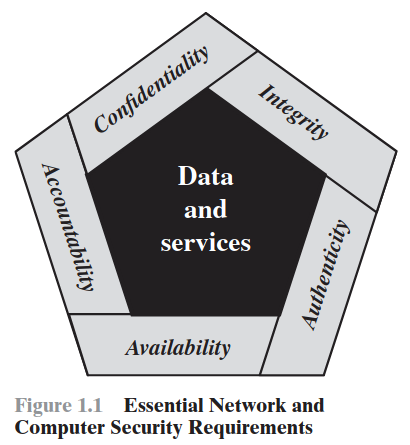
\includegraphics[width=0.5\linewidth]{Figuras/Figure1.1.png}






\end{frame}





